% Options for packages loaded elsewhere
\PassOptionsToPackage{unicode}{hyperref}
\PassOptionsToPackage{hyphens}{url}
%
\documentclass[
  ignorenonframetext,
]{beamer}
\usepackage{pgfpages}
\setbeamertemplate{caption}[numbered]
\setbeamertemplate{caption label separator}{: }
\setbeamercolor{caption name}{fg=normal text.fg}
\beamertemplatenavigationsymbolsempty
% Prevent slide breaks in the middle of a paragraph
\widowpenalties 1 10000
\raggedbottom
\setbeamertemplate{part page}{
  \centering
  \begin{beamercolorbox}[sep=16pt,center]{part title}
    \usebeamerfont{part title}\insertpart\par
  \end{beamercolorbox}
}
\setbeamertemplate{section page}{
  \centering
  \begin{beamercolorbox}[sep=12pt,center]{part title}
    \usebeamerfont{section title}\insertsection\par
  \end{beamercolorbox}
}
\setbeamertemplate{subsection page}{
  \centering
  \begin{beamercolorbox}[sep=8pt,center]{part title}
    \usebeamerfont{subsection title}\insertsubsection\par
  \end{beamercolorbox}
}
\AtBeginPart{
  \frame{\partpage}
}
\AtBeginSection{
  \ifbibliography
  \else
    \frame{\sectionpage}
  \fi
}
\AtBeginSubsection{
  \frame{\subsectionpage}
}
\usepackage{lmodern}
\usepackage{amssymb,amsmath}
\usepackage{ifxetex,ifluatex}
\ifnum 0\ifxetex 1\fi\ifluatex 1\fi=0 % if pdftex
  \usepackage[T1]{fontenc}
  \usepackage[utf8]{inputenc}
  \usepackage{textcomp} % provide euro and other symbols
\else % if luatex or xetex
  \usepackage{unicode-math}
  \defaultfontfeatures{Scale=MatchLowercase}
  \defaultfontfeatures[\rmfamily]{Ligatures=TeX,Scale=1}
\fi
% Use upquote if available, for straight quotes in verbatim environments
\IfFileExists{upquote.sty}{\usepackage{upquote}}{}
\IfFileExists{microtype.sty}{% use microtype if available
  \usepackage[]{microtype}
  \UseMicrotypeSet[protrusion]{basicmath} % disable protrusion for tt fonts
}{}
\makeatletter
\@ifundefined{KOMAClassName}{% if non-KOMA class
  \IfFileExists{parskip.sty}{%
    \usepackage{parskip}
  }{% else
    \setlength{\parindent}{0pt}
    \setlength{\parskip}{6pt plus 2pt minus 1pt}}
}{% if KOMA class
  \KOMAoptions{parskip=half}}
\makeatother
\usepackage{xcolor}
\IfFileExists{xurl.sty}{\usepackage{xurl}}{} % add URL line breaks if available
\IfFileExists{bookmark.sty}{\usepackage{bookmark}}{\usepackage{hyperref}}
\hypersetup{
  pdftitle={What's the FREQ?},
  pdfauthor={Lab 1G},
  hidelinks,
  pdfcreator={LaTeX via pandoc}}
\urlstyle{same} % disable monospaced font for URLs
\newif\ifbibliography
\usepackage{color}
\usepackage{fancyvrb}
\newcommand{\VerbBar}{|}
\newcommand{\VERB}{\Verb[commandchars=\\\{\}]}
\DefineVerbatimEnvironment{Highlighting}{Verbatim}{commandchars=\\\{\}}
% Add ',fontsize=\small' for more characters per line
\usepackage{framed}
\definecolor{shadecolor}{RGB}{248,248,248}
\newenvironment{Shaded}{\begin{snugshade}}{\end{snugshade}}
\newcommand{\AlertTok}[1]{\textcolor[rgb]{0.94,0.16,0.16}{#1}}
\newcommand{\AnnotationTok}[1]{\textcolor[rgb]{0.56,0.35,0.01}{\textbf{\textit{#1}}}}
\newcommand{\AttributeTok}[1]{\textcolor[rgb]{0.77,0.63,0.00}{#1}}
\newcommand{\BaseNTok}[1]{\textcolor[rgb]{0.00,0.00,0.81}{#1}}
\newcommand{\BuiltInTok}[1]{#1}
\newcommand{\CharTok}[1]{\textcolor[rgb]{0.31,0.60,0.02}{#1}}
\newcommand{\CommentTok}[1]{\textcolor[rgb]{0.56,0.35,0.01}{\textit{#1}}}
\newcommand{\CommentVarTok}[1]{\textcolor[rgb]{0.56,0.35,0.01}{\textbf{\textit{#1}}}}
\newcommand{\ConstantTok}[1]{\textcolor[rgb]{0.00,0.00,0.00}{#1}}
\newcommand{\ControlFlowTok}[1]{\textcolor[rgb]{0.13,0.29,0.53}{\textbf{#1}}}
\newcommand{\DataTypeTok}[1]{\textcolor[rgb]{0.13,0.29,0.53}{#1}}
\newcommand{\DecValTok}[1]{\textcolor[rgb]{0.00,0.00,0.81}{#1}}
\newcommand{\DocumentationTok}[1]{\textcolor[rgb]{0.56,0.35,0.01}{\textbf{\textit{#1}}}}
\newcommand{\ErrorTok}[1]{\textcolor[rgb]{0.64,0.00,0.00}{\textbf{#1}}}
\newcommand{\ExtensionTok}[1]{#1}
\newcommand{\FloatTok}[1]{\textcolor[rgb]{0.00,0.00,0.81}{#1}}
\newcommand{\FunctionTok}[1]{\textcolor[rgb]{0.00,0.00,0.00}{#1}}
\newcommand{\ImportTok}[1]{#1}
\newcommand{\InformationTok}[1]{\textcolor[rgb]{0.56,0.35,0.01}{\textbf{\textit{#1}}}}
\newcommand{\KeywordTok}[1]{\textcolor[rgb]{0.13,0.29,0.53}{\textbf{#1}}}
\newcommand{\NormalTok}[1]{#1}
\newcommand{\OperatorTok}[1]{\textcolor[rgb]{0.81,0.36,0.00}{\textbf{#1}}}
\newcommand{\OtherTok}[1]{\textcolor[rgb]{0.56,0.35,0.01}{#1}}
\newcommand{\PreprocessorTok}[1]{\textcolor[rgb]{0.56,0.35,0.01}{\textit{#1}}}
\newcommand{\RegionMarkerTok}[1]{#1}
\newcommand{\SpecialCharTok}[1]{\textcolor[rgb]{0.00,0.00,0.00}{#1}}
\newcommand{\SpecialStringTok}[1]{\textcolor[rgb]{0.31,0.60,0.02}{#1}}
\newcommand{\StringTok}[1]{\textcolor[rgb]{0.31,0.60,0.02}{#1}}
\newcommand{\VariableTok}[1]{\textcolor[rgb]{0.00,0.00,0.00}{#1}}
\newcommand{\VerbatimStringTok}[1]{\textcolor[rgb]{0.31,0.60,0.02}{#1}}
\newcommand{\WarningTok}[1]{\textcolor[rgb]{0.56,0.35,0.01}{\textbf{\textit{#1}}}}
\usepackage{graphicx,grffile}
\makeatletter
\def\maxwidth{\ifdim\Gin@nat@width>\linewidth\linewidth\else\Gin@nat@width\fi}
\def\maxheight{\ifdim\Gin@nat@height>\textheight\textheight\else\Gin@nat@height\fi}
\makeatother
% Scale images if necessary, so that they will not overflow the page
% margins by default, and it is still possible to overwrite the defaults
% using explicit options in \includegraphics[width, height, ...]{}
\setkeys{Gin}{width=\maxwidth,height=\maxheight,keepaspectratio}
% Set default figure placement to htbp
\makeatletter
\def\fps@figure{htbp}
\makeatother
\setlength{\emergencystretch}{3em} % prevent overfull lines
\providecommand{\tightlist}{%
  \setlength{\itemsep}{0pt}\setlength{\parskip}{0pt}}
\setcounter{secnumdepth}{-\maxdimen} % remove section numbering

\title{What's the FREQ?}
\author{Lab 1G}
\date{Directions: Follow along with the slides and answer the questions in
\textbf{red} font in your journal.}

\begin{document}
\frame{\titlepage}

\begin{frame}[fragile]{Clean it up!}
\protect\hypertarget{clean-it-up}{}

\begin{itemize}
\tightlist
\item
  In Lab 1F, we saw how we could \emph{clean} data to make it easier to
  use and analyze.

  \begin{itemize}
  \tightlist
  \item
    You cleaned a small set of variables from the American Time Use
    (ATU) survey.
  \item
    The process of cleaning and then analyzing data is \emph{very}
    common in Data Science.
  \end{itemize}
\item
  In this lab, we'll learn how we can create frequency tables to detect
  relationships between categorical variables.

  \begin{itemize}
  \tightlist
  \item
    For the sake of consistency, rather than using the data that you
    cleaned, you will use the pre-loaded ATU data.
  \item
    Use the \texttt{data()} function to load the \texttt{atu\_clean}
    data file to use in this lab.
  \end{itemize}
\end{itemize}

\end{frame}

\begin{frame}{How do we summarize categorical variables?}
\protect\hypertarget{how-do-we-summarize-categorical-variables}{}

\begin{itemize}
\tightlist
\item
  When we're dealing with categorical variables, we can't just calculate
  an \textbf{average} to describe a \emph{typical} value.

  \begin{itemize}
  \tightlist
  \item
    (Honestly, what's the average of categories \emph{orange},
    \emph{apple} and \emph{banana}, for instance?)
  \end{itemize}
\item
  When trying to describe categorical variables with numbers, we
  calculate \textbf{frequency tables}
\end{itemize}

\end{frame}

\begin{frame}[fragile]{Frequency tables?}
\protect\hypertarget{frequency-tables}{}

\begin{itemize}
\tightlist
\item
  When it comes to categories, about all you can do is \emph{count} or
  \emph{tally} how often each category comes up in the data.
\item
  Fill in the blanks below to answer the following: \textbf{How many
  more \emph{females} than \emph{males} are there in our ATU data?}
\end{itemize}

\begin{Shaded}
\begin{Highlighting}[]
\KeywordTok{tally}\NormalTok{(}\OperatorTok{~}\StringTok{ }\NormalTok{____, }\DataTypeTok{data =}\NormalTok{ ____)}
\end{Highlighting}
\end{Shaded}

\end{frame}

\begin{frame}[fragile]{2-way Frequency Tables}
\protect\hypertarget{way-frequency-tables}{}

\begin{itemize}
\tightlist
\item
  Counting the categories of a single variable is nice, but often times
  we want to make comparisons.
\item
  For example, what if we wanted to answer the question:

  \begin{itemize}
  \tightlist
  \item
    \textbf{Does one \texttt{gender} seem to have a higher occurrence of
    physical challenges than the other? If so, which one and explain
    your reasoning?}
  \end{itemize}
\item
  We could use the following plot to try and answer this question:
\end{itemize}

\begin{Shaded}
\begin{Highlighting}[]
\KeywordTok{bargraph}\NormalTok{(}\OperatorTok{~}\NormalTok{phys_challenge }\OperatorTok{|}\StringTok{ }\NormalTok{gender, }\DataTypeTok{data =}\NormalTok{ atu_clean)}
\end{Highlighting}
\end{Shaded}

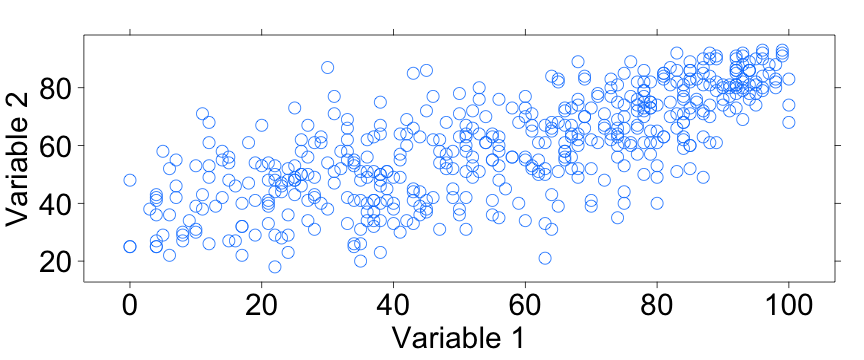
\includegraphics{lab1gRev_files/figure-beamer/unnamed-chunk-3-1.pdf}

\begin{itemize}
\tightlist
\item
  The split bargraph helps us get and idea of the answer to the
  question, but we need to provide precise values.
\item
  \textbf{Use a line of code, that's similar to how we facet plots, to
  obtain a tally of the number of people with physical challenges and
  their genders.}
\end{itemize}

\end{frame}

\begin{frame}[fragile]{Interpreting 2-way frequency tables}
\protect\hypertarget{interpreting-2-way-frequency-tables}{}

\begin{itemize}
\tightlist
\item
  Recall that there were 1153 more women than men in our data set.

  \begin{itemize}
  \tightlist
  \item
    If there are more women, then we might expect women to have more
    physical challenges (compared to men).
  \end{itemize}
\item
  Instead of using \emph{counts} we use \emph{percentages}.
\item
  Include: \texttt{format\ =\ "percent"} as an option to the code you
  used to make your 2-way frequency table. Then answer this question
  again:

  \begin{itemize}
  \tightlist
  \item
    \textbf{Does one \texttt{gender} seem to have a higher occurrence of
    physical challenges than the other? If so, which one and explain
    your reasoning?}
  \item
    \textbf{Did your answer change from before? Why?}
  \end{itemize}
\item
  It's often helpful to display totals in our 2-way frequency tables.

  \begin{itemize}
  \tightlist
  \item
    To include them, include \texttt{margins\ =\ TRUE} as an option in
    the tally function.
  \end{itemize}
\end{itemize}

\end{frame}

\begin{frame}[fragile]{Conditional Relative Frequencies}
\protect\hypertarget{conditional-relative-frequencies}{}

\begin{itemize}
\tightlist
\item
  There is as difference between
  \texttt{phys\_challenge\ \textbar{}\ gender} and
  \texttt{gender\ \textbar{}\ phys\_challenge}.
\end{itemize}

\begin{Shaded}
\begin{Highlighting}[]
\KeywordTok{tally}\NormalTok{(}\OperatorTok{~}\NormalTok{phys_challenge }\OperatorTok{|}\StringTok{ }\NormalTok{gender, }\DataTypeTok{data =}\NormalTok{ atu_clean, }\DataTypeTok{margin =} \OtherTok{TRUE}\NormalTok{)}
\end{Highlighting}
\end{Shaded}

\begin{verbatim}
##                 gender
## phys_challenge   Male Female
##   No difficulty  4140   5048
##   Has difficulty  530    775
##   Total          4670   5823
\end{verbatim}

\begin{Shaded}
\begin{Highlighting}[]
\KeywordTok{tally}\NormalTok{(}\OperatorTok{~}\NormalTok{gender }\OperatorTok{|}\StringTok{ }\NormalTok{phys_challenge, }\DataTypeTok{data =}\NormalTok{ atu_clean, }\DataTypeTok{margin =} \OtherTok{TRUE}\NormalTok{)}
\end{Highlighting}
\end{Shaded}

\begin{verbatim}
##         phys_challenge
## gender   No difficulty Has difficulty
##   Male            4140            530
##   Female          5048            775
##   Total           9188           1305
\end{verbatim}

\begin{itemize}
\item
  At first glance, the two-way frequency tables might look similar
  (especially when the \texttt{margin} option is excluded). Notice,
  however, that the totals are different.
\item
  The totals are telling us that \texttt{R} calculates conditional
  frequencies by column!
\item
  What does this mean?

  \begin{itemize}
  \tightlist
  \item
    The first two-way frequency tables is comparing males and females
    and the distribution of physical challenges.
  \item
    The second is comparing people with no physical challenges and those
    with physical challenges and the distribution of gender among each
    group.
  \end{itemize}
\item
  \textbf{Add the option \texttt{format\ =\ "percent"} to each tally
  function. How were the percents calculated?}
\end{itemize}

\end{frame}

\begin{frame}{On your own}
\protect\hypertarget{on-your-own}{}

\begin{itemize}
\tightlist
\item
  \textbf{Describe what happens if you create a 2-way frequency table
  with a numerical variable and a categorical variable.}
\item
  \textbf{How are the types of statistical questions that 2-way
  frequency tables can answer different than 1-way frequency tables?}
\item
  \textbf{Which gender has a higher rate of \emph{part time
  employment}?}
\end{itemize}

\end{frame}

\end{document}
